\documentclass[11pt,a4paper]{article}

\usepackage[T1]{fontenc}
\usepackage[utf8]{inputenc}
\usepackage[brazil]{babel}
\usepackage[margin=2.2cm]{geometry}
\usepackage{graphicx}
\usepackage{float}
\usepackage{booktabs}
\usepackage{caption}
\usepackage{xcolor}
\usepackage[colorlinks=true,linkcolor=black,urlcolor=black]{hyperref}

\captionsetup{font=small,labelfont=bf}
% As figuras vivem em results/figures, geradas por src/analysis. Este
% documento apenas as reúne e comenta; não as reproduz.
\graphicspath{
    {../../results/figures/dataset/}
    {../../results/figures/folds/}
    {../../results/figures/hdbscan/}
}

\setlength{\parskip}{0.6em}
\setlength{\parindent}{0pt}

\title{\textbf{Atlas de figuras}\\[0.3em]
\large Análise exploratória da base, das partições e dos resultados do HDBSCAN}
\author{Heitor Rodrigues Sabino}
\date{Setembro de 2026}

\begin{document}

\maketitle

\section*{Sobre este documento}

Reúne as treze figuras produzidas pelos scripts em \texttt{src/analysis/},
explicando o que cada uma mostra, como lê-la e o que ela significa para o
trabalho. As figuras são geradas por código versionado, não montadas à mão:

\begin{verbatim}
python src/analysis/dataset_analysis.py   # results/figures/dataset
python src/analysis/fold_analysis.py      # results/figures/folds
python src/analysis/hdbscan_metrics.py    # results/figures/hdbscan
\end{verbatim}

\paragraph{Uma decisão que atravessa todas as figuras.}
O poder discriminante é medido por \textbf{AUPRC} (precisão média), nunca por
AUC ROC. Com 0,172\% de fraudes, o AUC ROC é dominado pela ordenação dos
284.315 negativos --- que não é a pergunta --- e reporta valores bem mais
generosos do que os dados sustentam. O AUPRC mede a precisão no topo do
ranking, que é o que importa quando apenas uma fração mínima das transações
será acusada.

Onde aparece o termo \emph{lift}, trata-se do AUPRC dividido pela prevalência,
isto é, pelo AUPRC de $0{,}001727$ que um ordenador aleatório obteria. Lift
igual a 1 significa nenhuma informação.

\vspace{1em}
\hrule
\vspace{1em}

\part*{Parte I --- A base de dados}
\addcontentsline{toc}{part}{Parte I --- A base de dados}

\section{Matriz de correlação}

\begin{figure}[H]
    \centering
    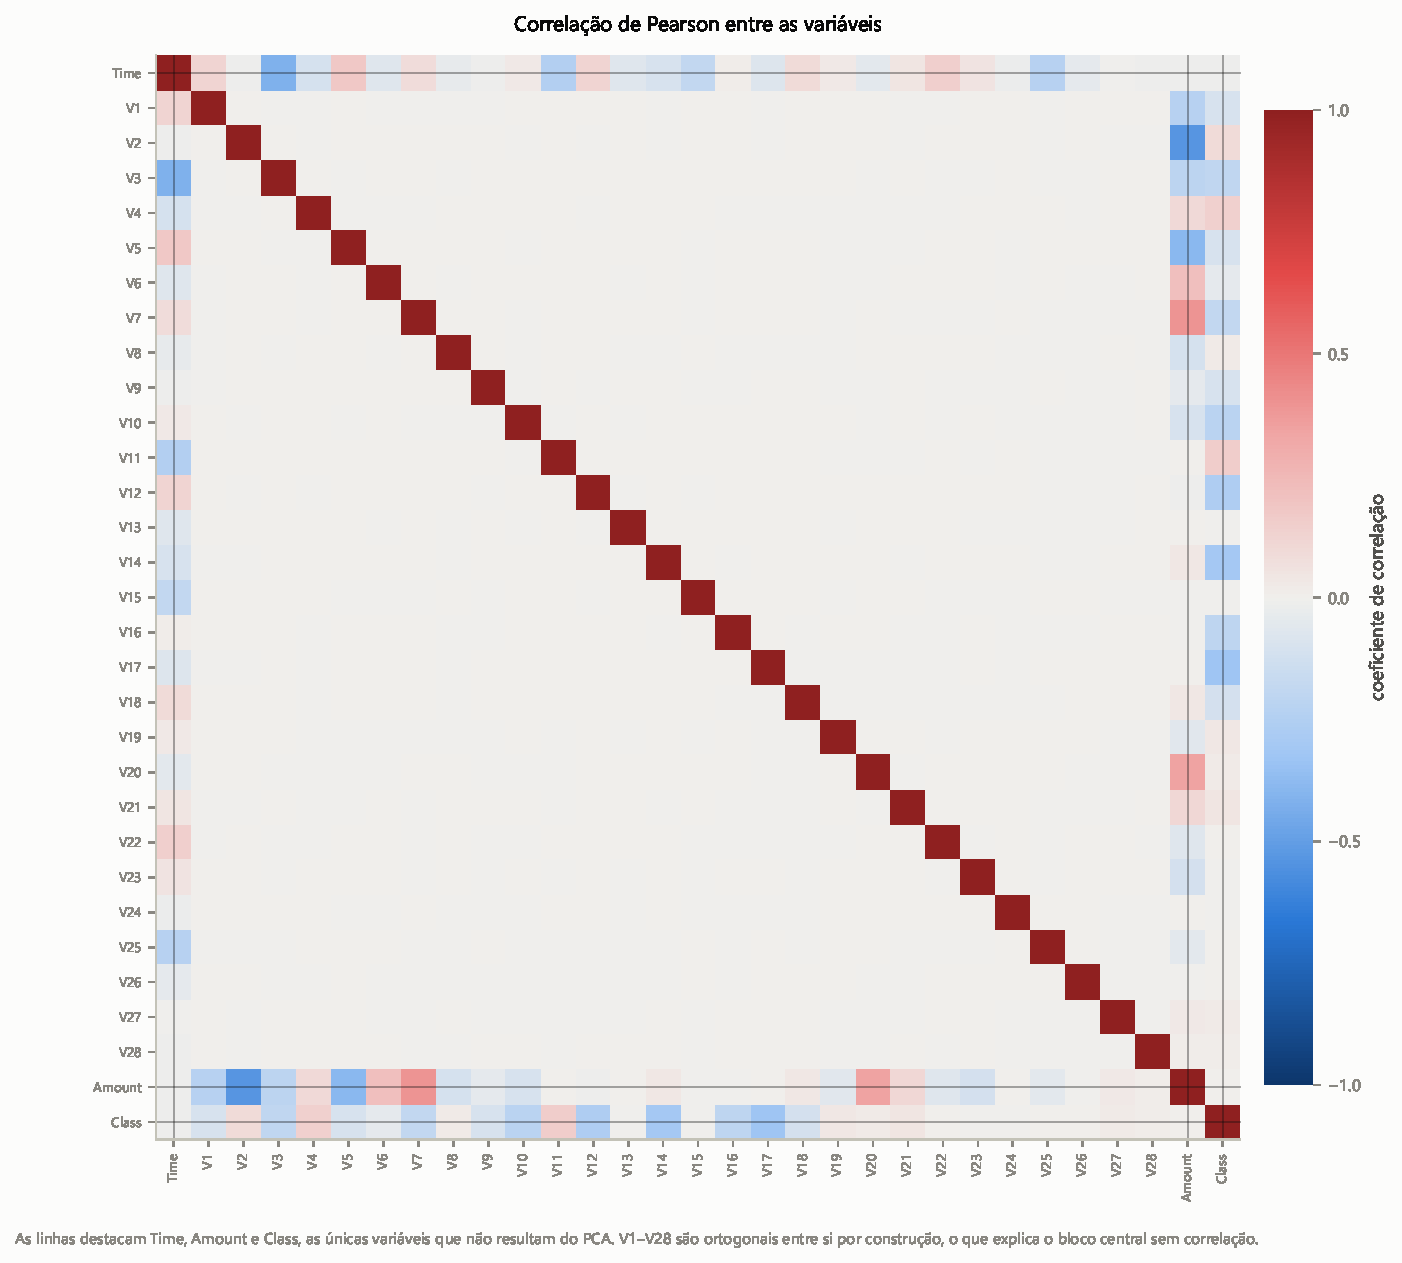
\includegraphics[width=0.86\textwidth]{01-correlation-matrix.pdf}
    \caption{Correlação de Pearson entre as 31 variáveis. As linhas escuras
    destacam \texttt{Time}, \texttt{Amount} e \texttt{Class}, as únicas que não
    resultam do PCA.}
\end{figure}

\textbf{Como ler.} Azul indica correlação negativa, vermelho indica positiva,
cinza indica ausência de correlação. A diagonal é sempre 1 por construção.

\textbf{O que mostra.} O bloco central é inteiramente neutro: as componentes
\texttt{V1}--\texttt{V28} não se correlacionam entre si. A correlação absoluta
máxima entre elas é de $2{,}32 \times 10^{-14}$, ou seja, zero numérico.

\textbf{O que significa.} A ortogonalidade é esperada, já que as componentes
principais são construídas justamente para serem não correlacionadas. A
consequência prática é que \textbf{nenhum tratamento de multicolinearidade é
necessário} --- decisão que a Metodologia registra e que esta figura
fundamenta. As únicas faixas com estrutura visível são as de \texttt{Time},
\texttt{Amount} e \texttt{Class}, que ficaram fora da transformação.

\section{Poder discriminante de cada variável}

\begin{figure}[H]
    \centering
    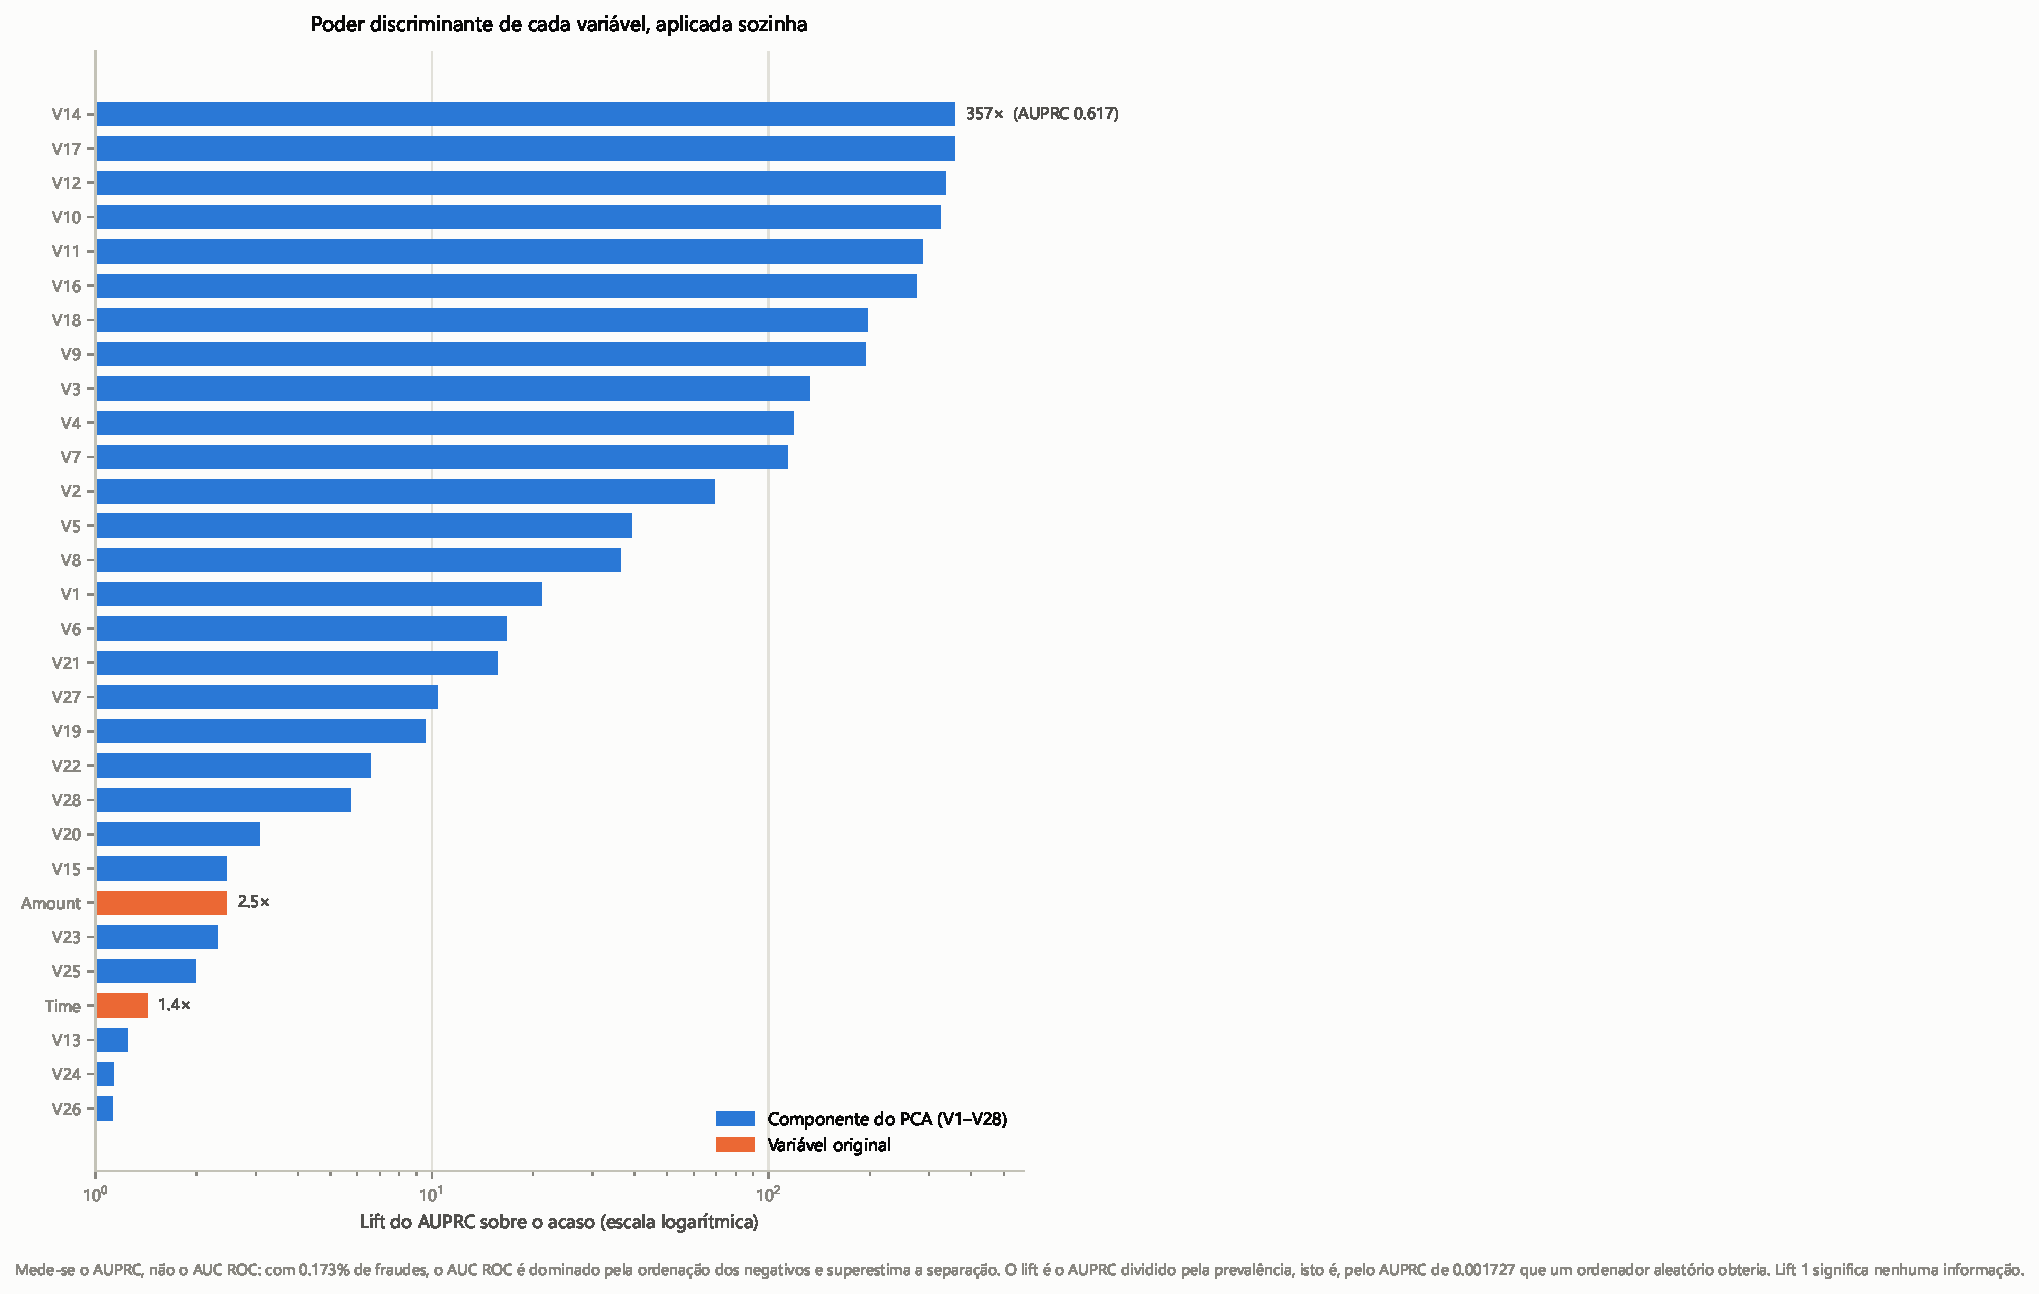
\includegraphics[width=0.80\textwidth]{02-feature-discriminative-power.pdf}
    \caption{Lift do AUPRC de cada variável aplicada isoladamente, em escala
    logarítmica. Em laranja, as duas variáveis originais.}
\end{figure}

\textbf{Como ler.} Cada barra mede quantas vezes a variável, sozinha, ordena
fraudes melhor que o acaso. A escala é logarítmica porque os valores variam
três ordens de grandeza. A linha em 1 marca o ordenador aleatório.

\textbf{O que mostra.} \texttt{V14} lidera com lift de 357$\times$
(AUPRC $0{,}617$), seguida de \texttt{V17} (356$\times$) e \texttt{V12}
(336$\times$). No extremo oposto, \texttt{Time} obtém apenas 1,43$\times$ e
\texttt{Amount}, 2,45$\times$.

\textbf{O que significa.} A escolha da métrica não é detalhe de forma. Medido
por AUC ROC, \texttt{V17} aparecia em oitavo lugar e \texttt{V4} em segundo; por
AUPRC, \texttt{V17} sobe para o segundo e \texttt{V4} cai para o décimo. A razão
é que \texttt{V4} ordena bem os negativos --- o que o AUC ROC premia --- mas não
coloca as fraudes no topo do ranking. \texttt{V17}, por sua vez, é a variável de
maior correlação absoluta com a classe ($-0{,}327$), e o AUC ROC a escondia.

\section{A variável \texttt{Time} é relevante?}

\begin{figure}[H]
    \centering
    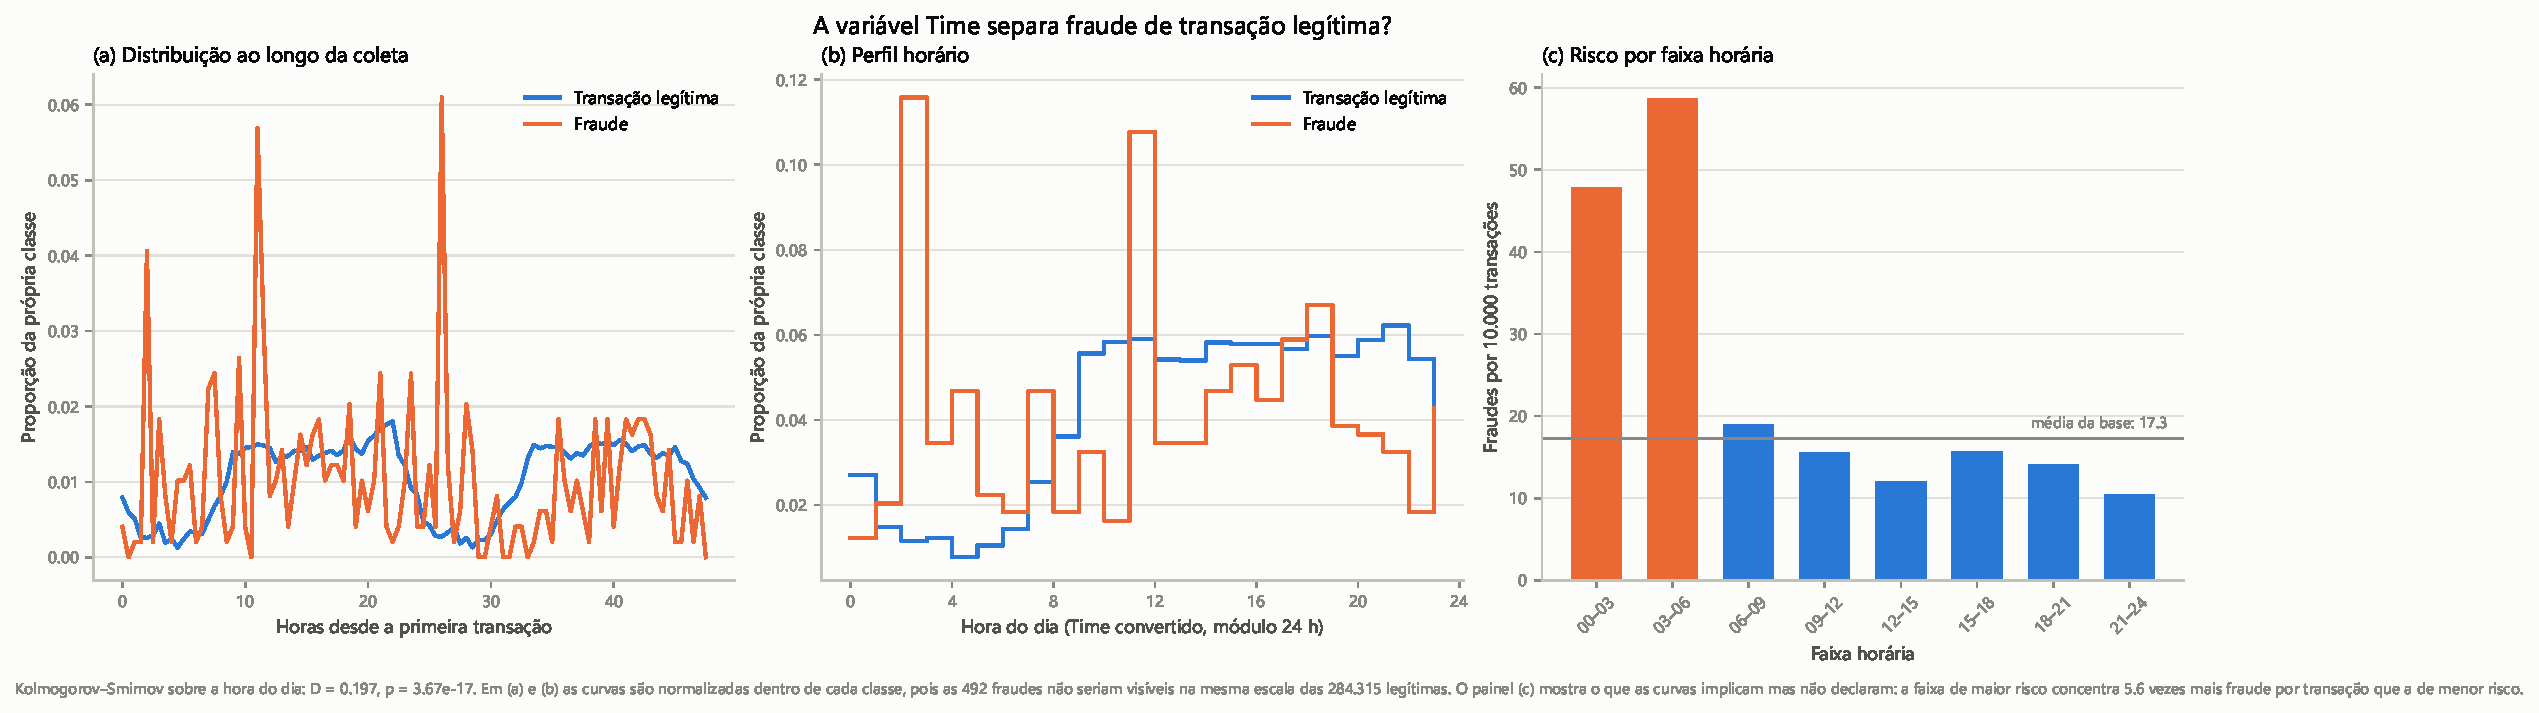
\includegraphics[width=\textwidth]{03-time-relevance.pdf}
    \caption{Distribuição temporal das duas classes ao longo das 48 horas de
    coleta (a), perfil por hora do dia (b) e taxa de fraude por faixa horária
    (c).}
\end{figure}

\textbf{Como ler.} Em (a) e (b) as curvas são normalizadas \emph{dentro de cada
classe}: sem isso, as 492 fraudes seriam invisíveis ao lado das 284.315
transações legítimas. O painel (c) muda de perspectiva e mostra, para cada faixa
de três horas, quantas fraudes ocorrem a cada 10.000 transações.

\textbf{O que mostra.} A resposta tem duas partes, e elas parecem contraditórias
até que se observe o que cada painel mede.

Como ordenador isolado, \texttt{Time} é quase inútil: AUPRC de $0{,}0025$, lift
de 1,43$\times$, 27ª posição entre 30 variáveis, correlação de $-0{,}012$ com a
classe.

Mas o painel (c) revela estrutura real. A faixa das 03h às 06h concentra
\textbf{58,7 fraudes por 10.000 transações}; a das 21h às 24h, apenas
\textbf{10,4}. Uma razão de 5,6 vezes.

\textbf{O que significa.} As duas leituras convivem porque medem coisas
diferentes. A hora do dia \emph{multiplica a probabilidade a priori} de fraude,
mas não serve para \emph{ordenar transações uma a uma} --- a maioria das
fraudes ocorre durante o dia, junto com a maioria das transações. A variável
bruta não merece entrar no modelo pelo seu poder isolado; a hora do dia
derivada dela é candidata legítima a variável construída.

\section{Distribuições por classe}

\begin{figure}[H]
    \centering
    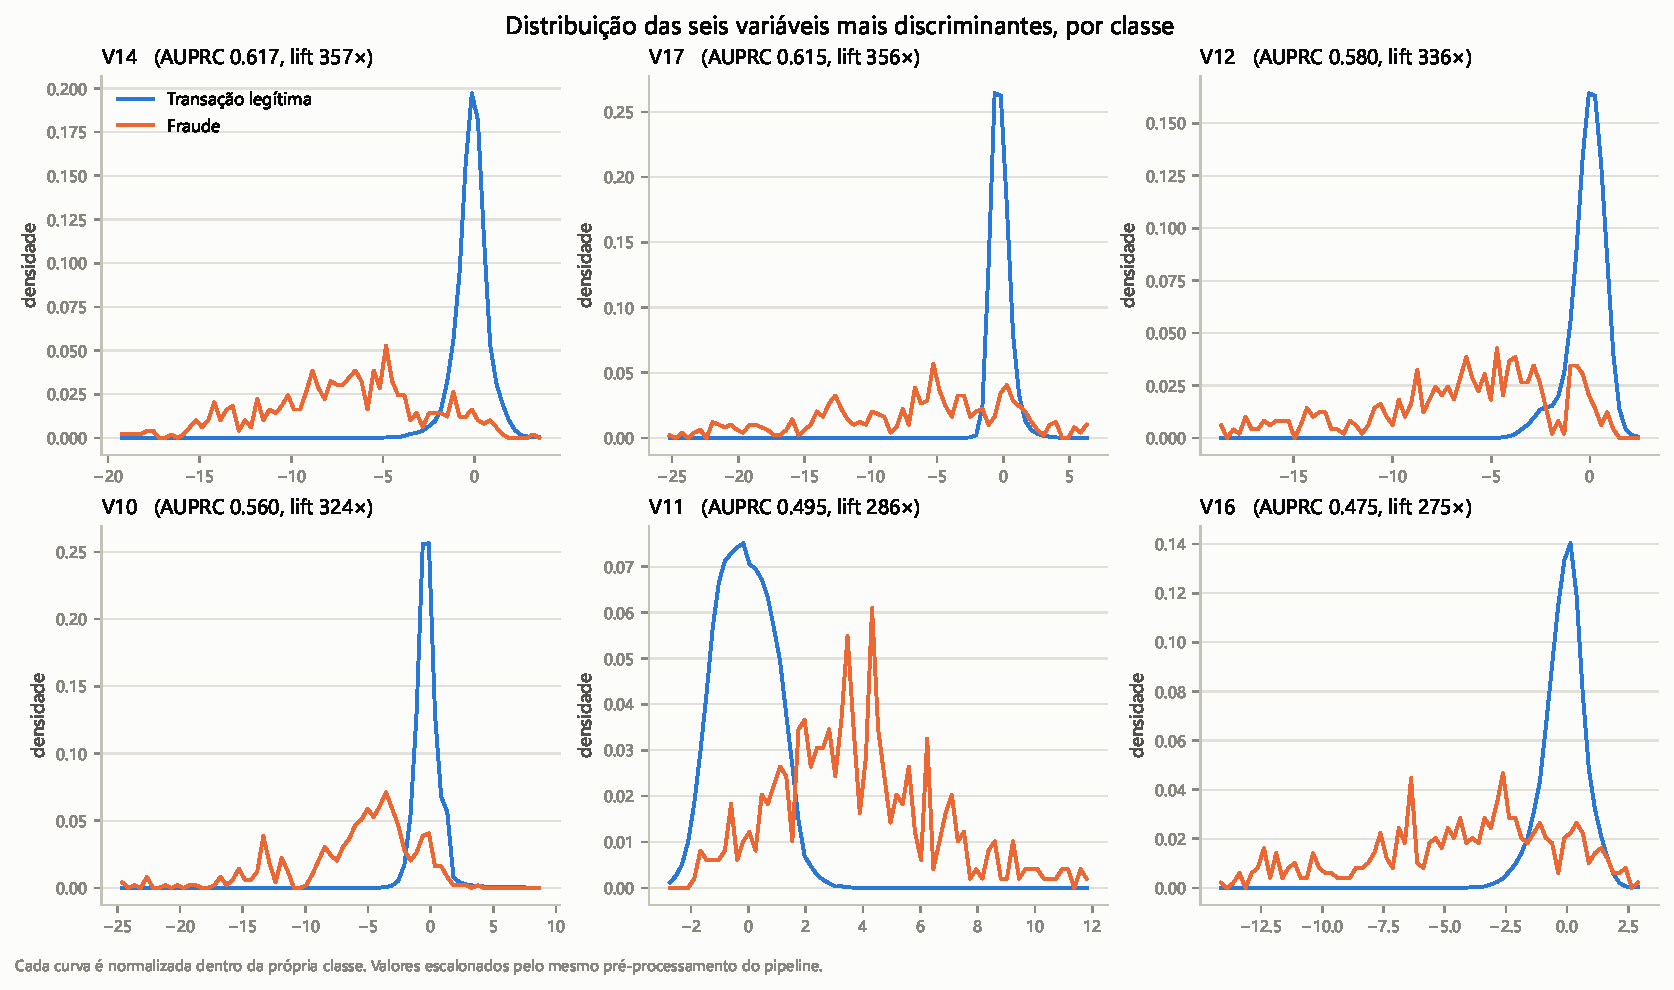
\includegraphics[width=\textwidth]{04-class-distributions.pdf}
    \caption{Distribuição das seis variáveis de maior AUPRC, separadas por
    classe. Valores escalonados pelo mesmo pré-processamento do pipeline.}
\end{figure}

\textbf{Como ler.} Cada curva é normalizada dentro da própria classe, de modo
que a comparação é de \emph{formato}, não de volume.

\textbf{O que mostra.} Em todas as seis variáveis as duas distribuições se
deslocam visivelmente uma em relação à outra, e em cinco delas a fraude desloca-se
para valores menores --- coerente com o sentido registrado na tabela de poder
discriminante.

\textbf{O que significa.} A separação existe, mas há sobreposição substancial em
todos os casos. Nenhuma variável isolada resolve o problema, o que justifica a
abordagem multivariada. Também explica por que o melhor AUPRC individual é
$0{,}617$ e não algo próximo de 1.

\section{Projeções bidimensionais}

\begin{figure}[H]
    \centering
    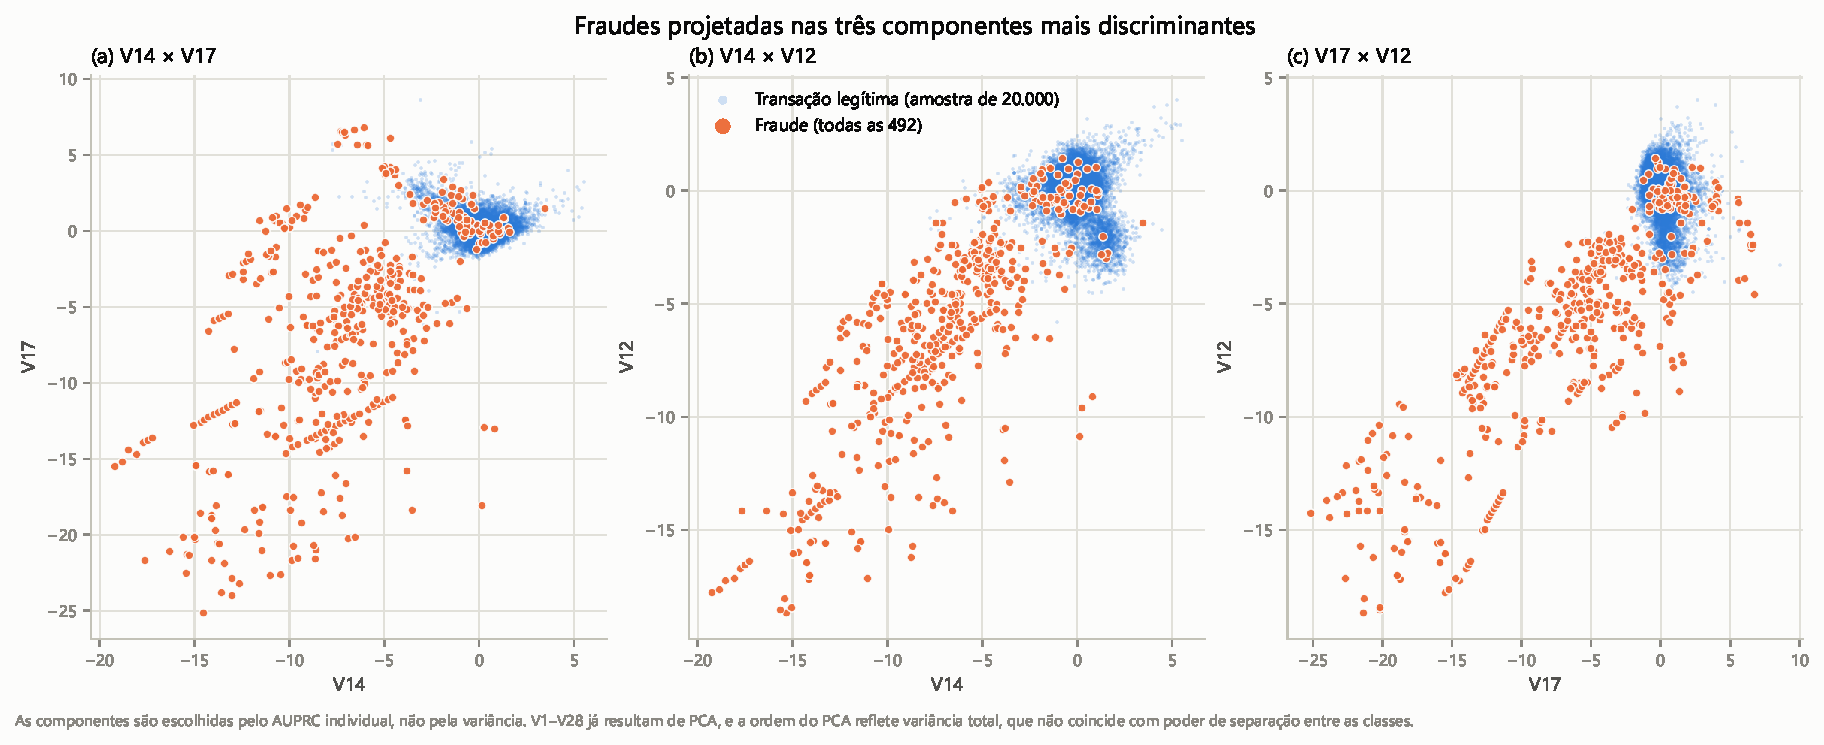
\includegraphics[width=\textwidth]{05-projections.pdf}
    \caption{Fraudes projetadas nos pares formados pelas três componentes de
    maior AUPRC.}
\end{figure}

\textbf{Como ler.} As transações legítimas aparecem em azul, como amostra de
20.000 pontos; as fraudes, em laranja, \emph{todas as 492}, desenhadas por cima
com anel de contorno. A subamostragem é necessária: com 284 mil pontos sobrepostos,
as fraudes ficariam soterradas.

\textbf{O que mostra.} As fraudes formam uma nuvem difusa que se estende para
fora do bloco denso das transações legítimas, com uma região de sobreposição
onde as duas classes convivem.

\textbf{O que significa.} Os eixos foram escolhidos pelo \textbf{AUPRC
individual, não pela variância}. Isso merece nota: as componentes já resultam de
PCA, e a ordem do PCA reflete variância total, que não coincide com poder de
separação entre classes. Projetar em \texttt{V1}, \texttt{V2} e \texttt{V3}
mostraria as direções de maior espalhamento, não as de maior informação sobre
fraude.

\section{Estrutura tridimensional}

\begin{figure}[H]
    \centering
    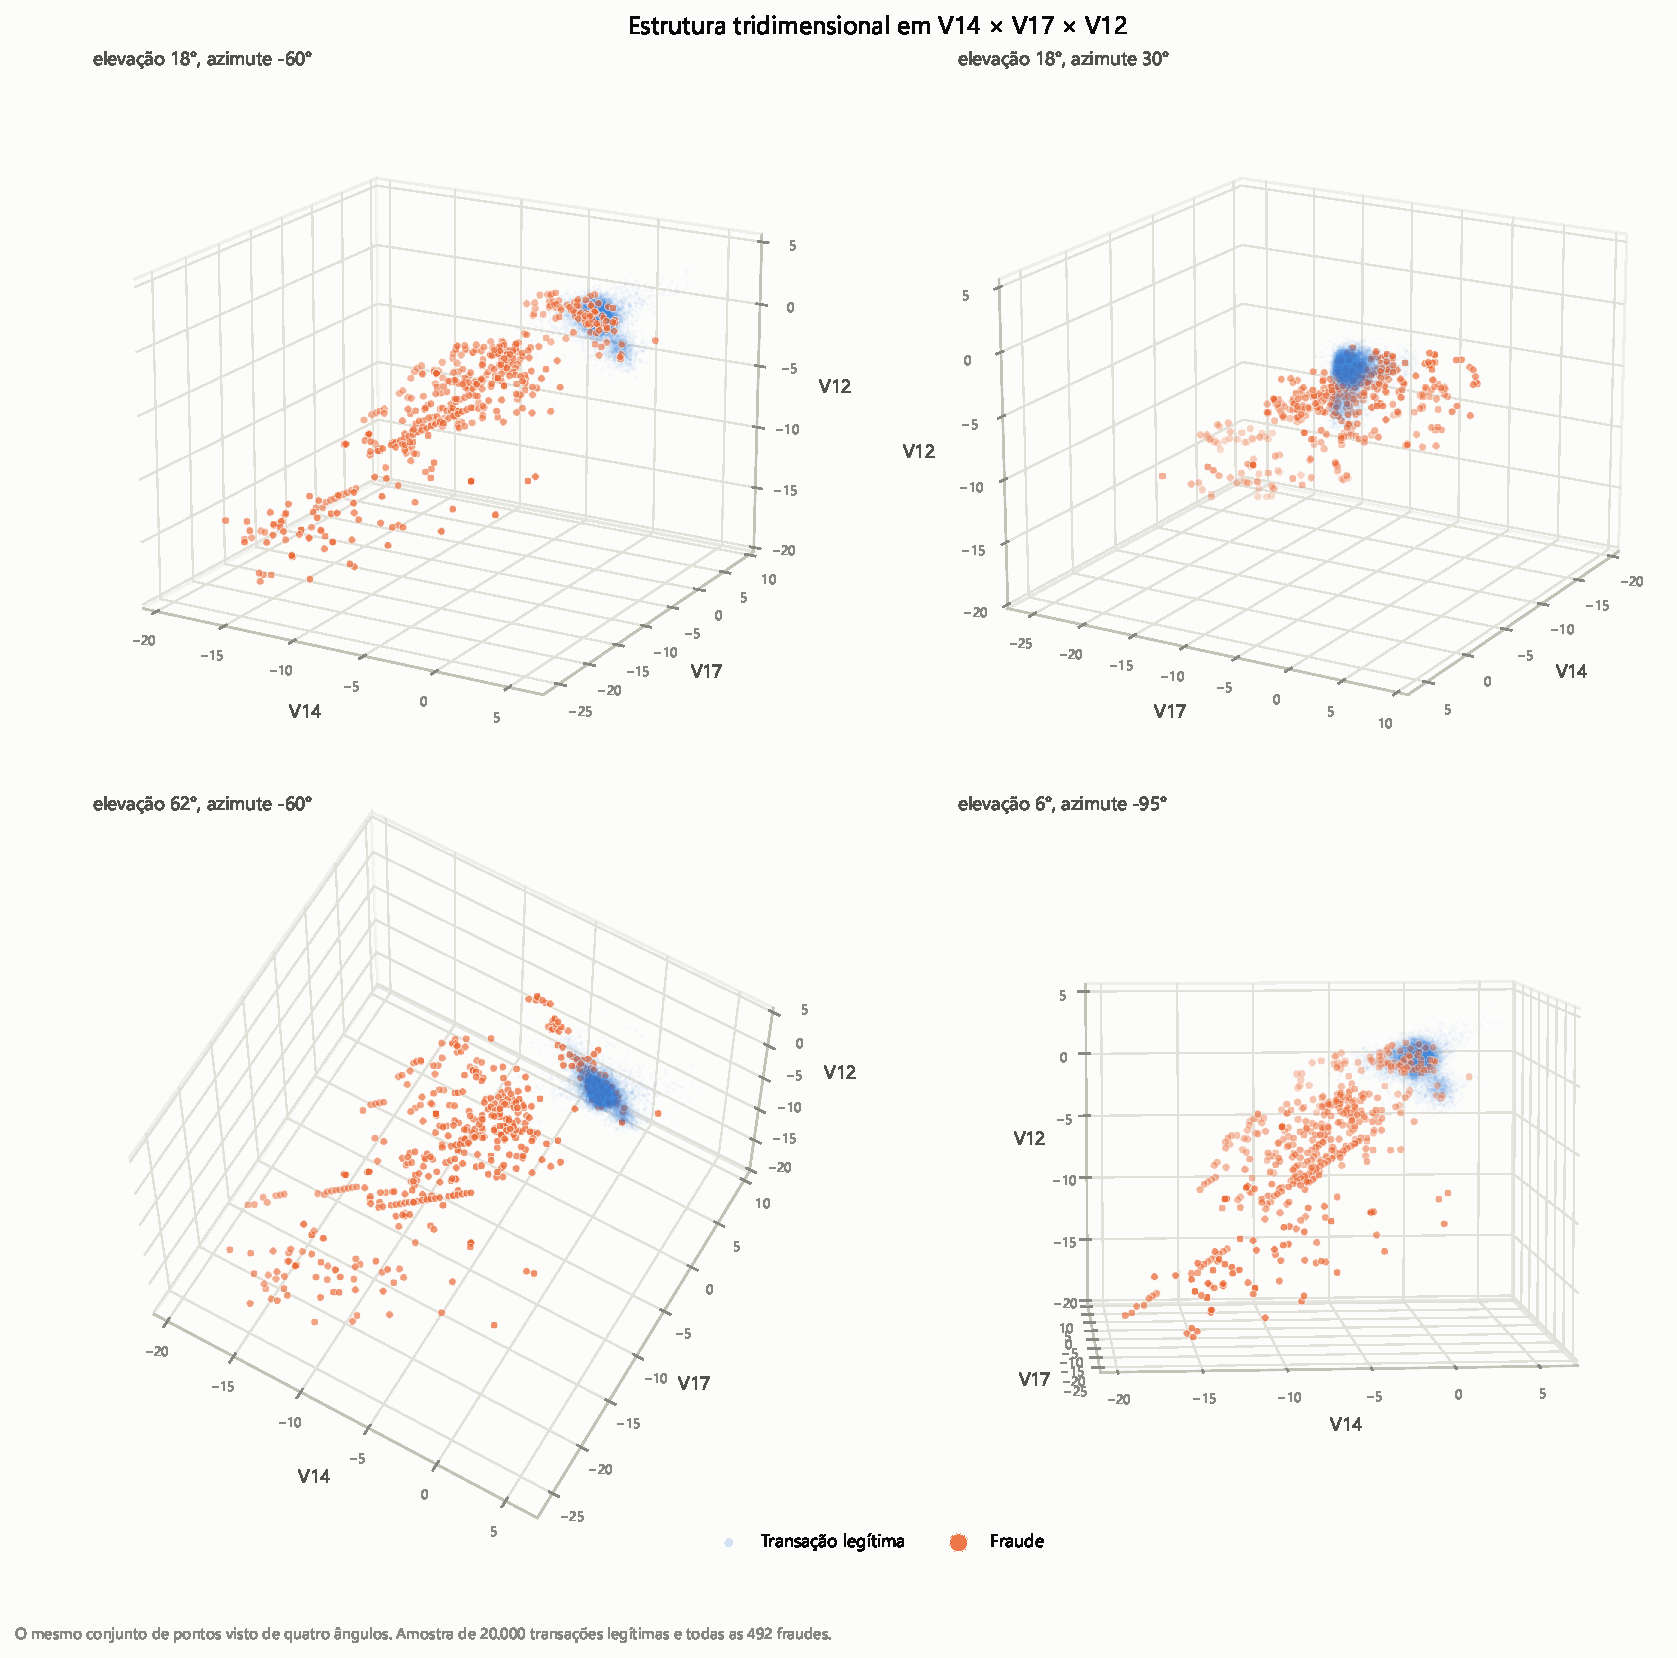
\includegraphics[width=0.92\textwidth]{06-projection-3d.pdf}
    \caption{A mesma nuvem de pontos vista de quatro ângulos, em
    \texttt{V14} $\times$ \texttt{V17} $\times$ \texttt{V12}.}
\end{figure}

\textbf{Como ler.} Os quatro painéis contêm exatamente os mesmos dados; só a
posição do observador muda.

\textbf{O que mostra.} A separação entre as duas nuvens persiste em todos os
ângulos. O bloco azul permanece compacto e a nuvem laranja permanece dispersa ao
seu redor, independentemente da direção de observação.

\textbf{O que significa.} Um único ângulo pode criar separação aparente por
oclusão --- pontos que apenas parecem separados porque estão alinhados com a
linha de visão. A rotação descarta esse artefato: a estrutura é genuína, não um
acidente de projeção.

\section{Densidade local: a premissa sob teste}

\begin{figure}[H]
    \centering
    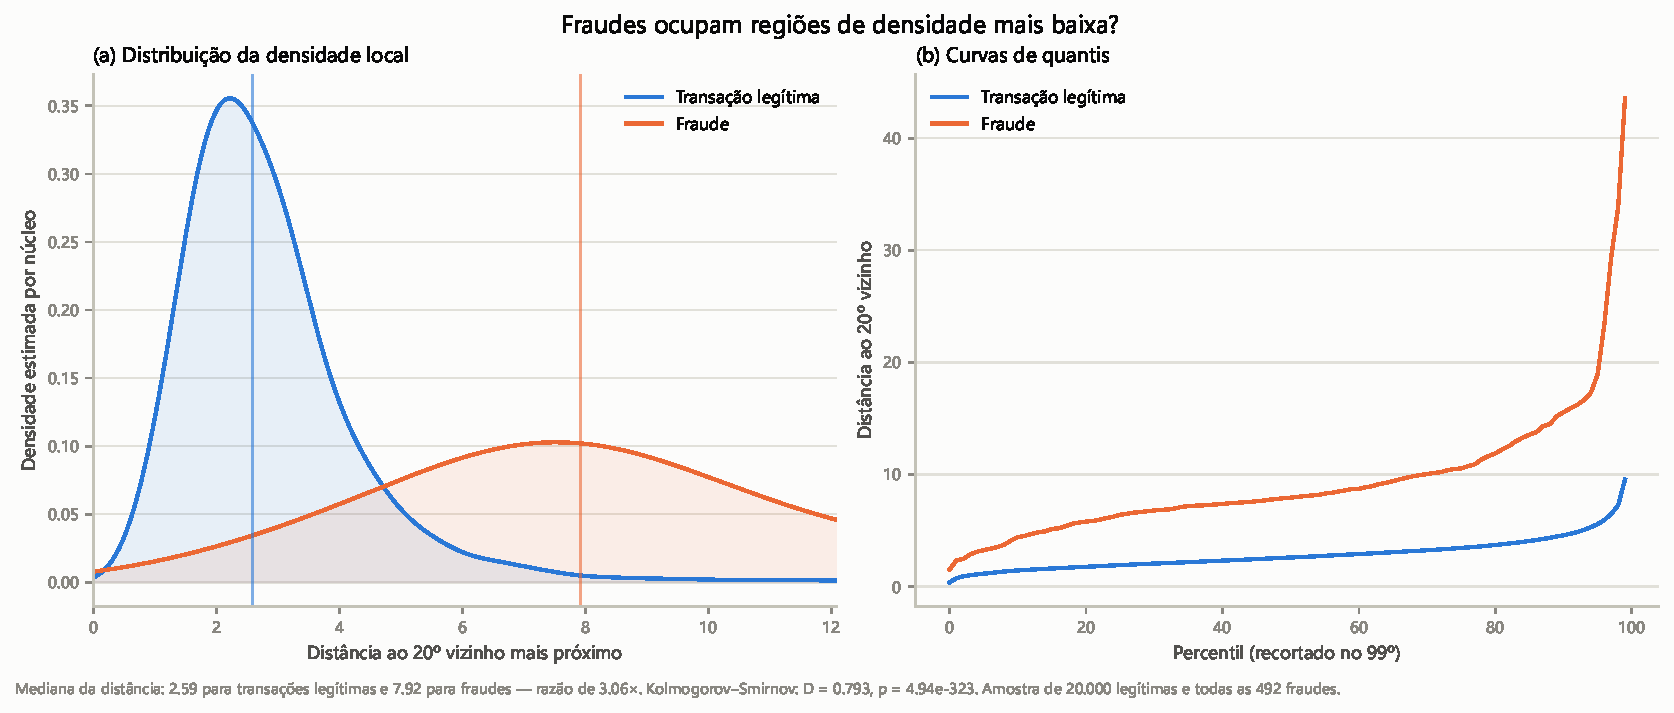
\includegraphics[width=\textwidth]{07-local-density.pdf}
    \caption{Distribuição da distância ao 20º vizinho mais próximo (a) e curvas
    de quantis das duas classes (b).}
\end{figure}

\textbf{Como ler.} A distância ao vigésimo vizinho é uma medida inversa de
densidade: quanto maior, mais isolado está o ponto. As linhas verticais em (a)
marcam as medianas. A densidade é estimada por núcleo, e não por histograma,
porque com apenas 492 fraudes um histograma seria dominado por ruído de
discretização.

\textbf{O que mostra.} As duas distribuições mal se sobrepõem. A distância
mediana é de $2{,}59$ para transações legítimas e de $7{,}92$ para fraudes ---
uma razão de \textbf{3,06 vezes}. O teste de Kolmogorov--Smirnov acusa
$D = 0{,}793$, com $p$ abaixo do menor valor representável em ponto flutuante.

\textbf{O que significa.} Esta é a figura mais importante do conjunto. Ela é a
\textbf{evidência empírica direta da premissa do trabalho}: fraudes de fato
ocupam regiões de baixa densidade. Sem esse resultado, tratar fraude como ruído
seria uma suposição não verificada; com ele, é uma propriedade mensurada da
base.

\clearpage
\part*{Parte II --- As partições da validação cruzada}
\addcontentsline{toc}{part}{Parte II --- As partições}

\section{Composição e estratificação}

\begin{figure}[H]
    \centering
    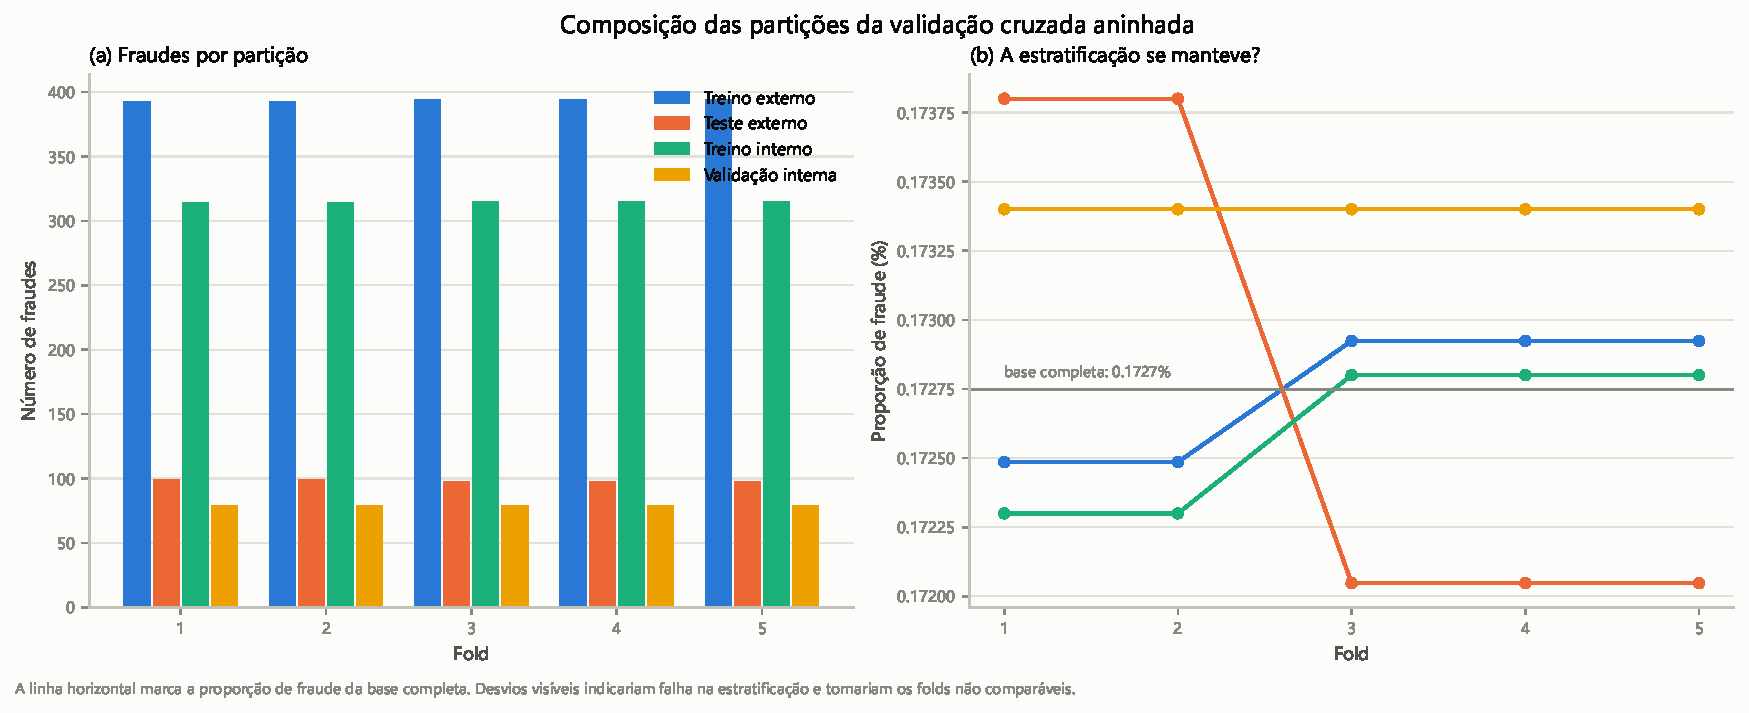
\includegraphics[width=\textwidth]{01-fold-composition.pdf}
    \caption{Número absoluto de fraudes por partição (a) e proporção de fraude
    em cada uma (b), comparada à da base completa.}
\end{figure}

\textbf{Como ler.} Em (b), a linha horizontal cinza marca a proporção de fraude
da base inteira. Qualquer desvio visível indicaria falha na estratificação.

\textbf{O que mostra.} As quatro séries permanecem praticamente coladas à linha
de referência. A proporção de fraude varia de $0{,}1720\%$ a $0{,}1738\%$ entre
todas as partições --- amplitude de $0{,}0018$ ponto percentual.

\textbf{O que significa.} A estratificação funcionou. Isso é pré-requisito para
comparar os folds entre si: se as partições tivessem proporções diferentes de
fraude, qualquer variação de desempenho poderia ser atribuída à composição, e
não ao modelo.

\section{Cobertura e isolamento}

\begin{figure}[H]
    \centering
    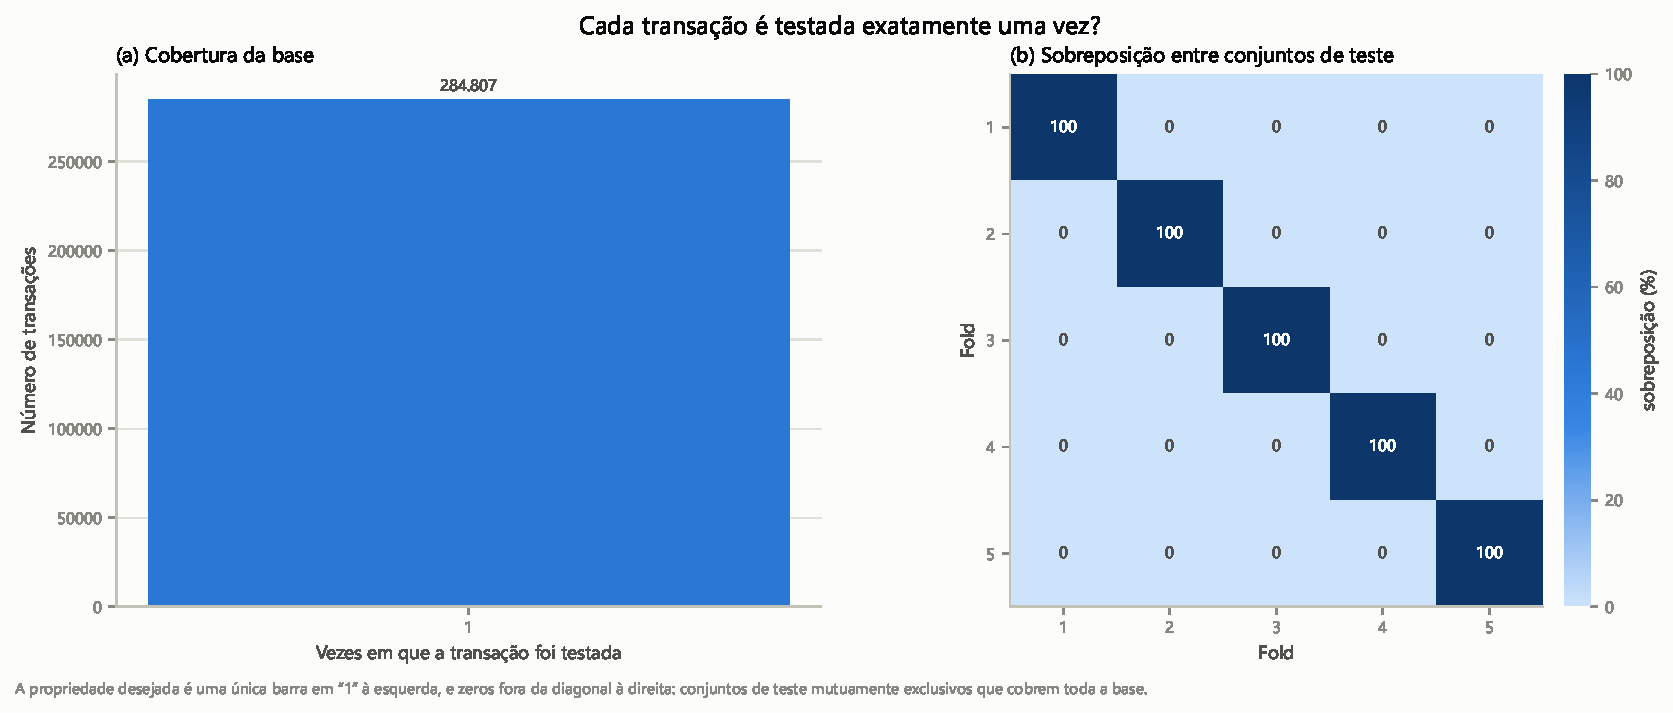
\includegraphics[width=\textwidth]{02-fold-coverage.pdf}
    \caption{Quantas vezes cada transação foi usada como teste (a) e
    sobreposição entre os conjuntos de teste dos cinco folds (b).}
\end{figure}

\textbf{Como ler.} A propriedade desejada é uma única barra em ``1'' à esquerda,
e zeros fora da diagonal à direita.

\textbf{O que mostra.} É exatamente o que se observa. Todas as
\textbf{284.807} transações foram testadas uma única vez, e a sobreposição entre
conjuntos de teste distintos é \textbf{nula}.

\textbf{O que significa.} Os conjuntos de teste são mutuamente exclusivos e
cobrem a base inteira. A estimativa de desempenho usa cada transação exatamente
uma vez, sem reaproveitamento --- que é a garantia que a validação cruzada
aninhada deve oferecer.

\section{Densidade das fraudes por fold}

\begin{figure}[H]
    \centering
    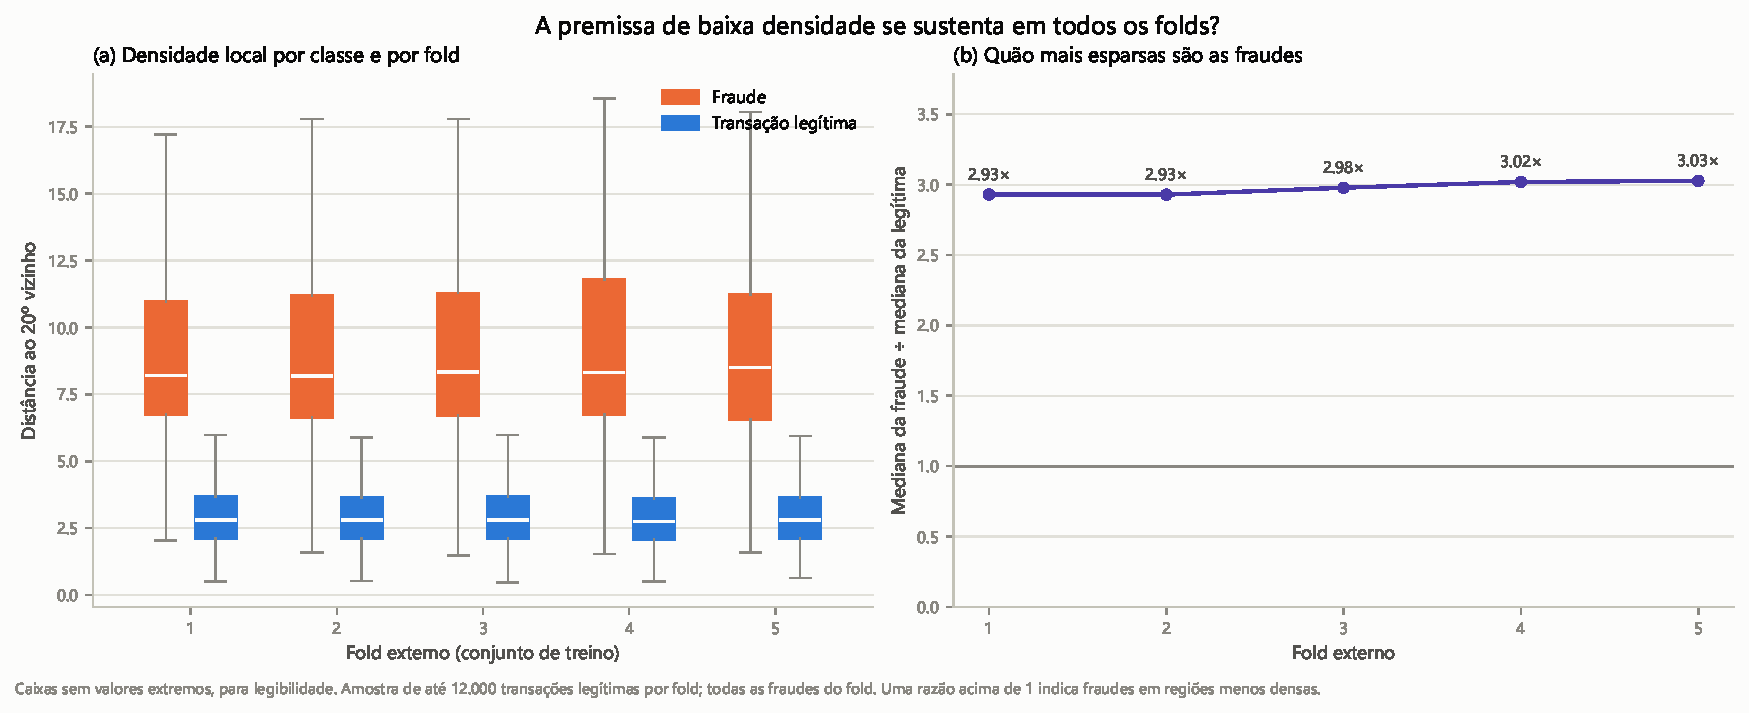
\includegraphics[width=\textwidth]{03-fraud-density-by-fold.pdf}
    \caption{Distribuição da densidade local por classe em cada fold (a) e razão
    entre as medianas das duas classes (b).}
\end{figure}

\textbf{Como ler.} Em (a), cada par de caixas compara as duas classes dentro de
um mesmo fold. Em (b), a razão acima de 1 indica fraudes em regiões menos densas.

\textbf{O que mostra.} A razão é \textbf{notavelmente estável}: $2{,}93\times$,
$2{,}93\times$, $2{,}98\times$, $3{,}02\times$ e $3{,}03\times$. Amplitude total
de $0{,}10$.

\textbf{O que significa.} Este resultado é decisivo para interpretar a
instabilidade do HDBSCAN, tratada na Parte III. Ele estabelece que \textbf{as
cinco partições são estruturalmente equivalentes} do ponto de vista da densidade.
Qualquer variação grande de resultado entre elas, portanto, não pode ser
atribuída a diferenças nos dados.

\clearpage
\part*{Parte III --- Resultados do HDBSCAN}
\addcontentsline{toc}{part}{Parte III --- Resultados do HDBSCAN}

\section{Estabilidade das métricas}

\begin{figure}[H]
    \centering
    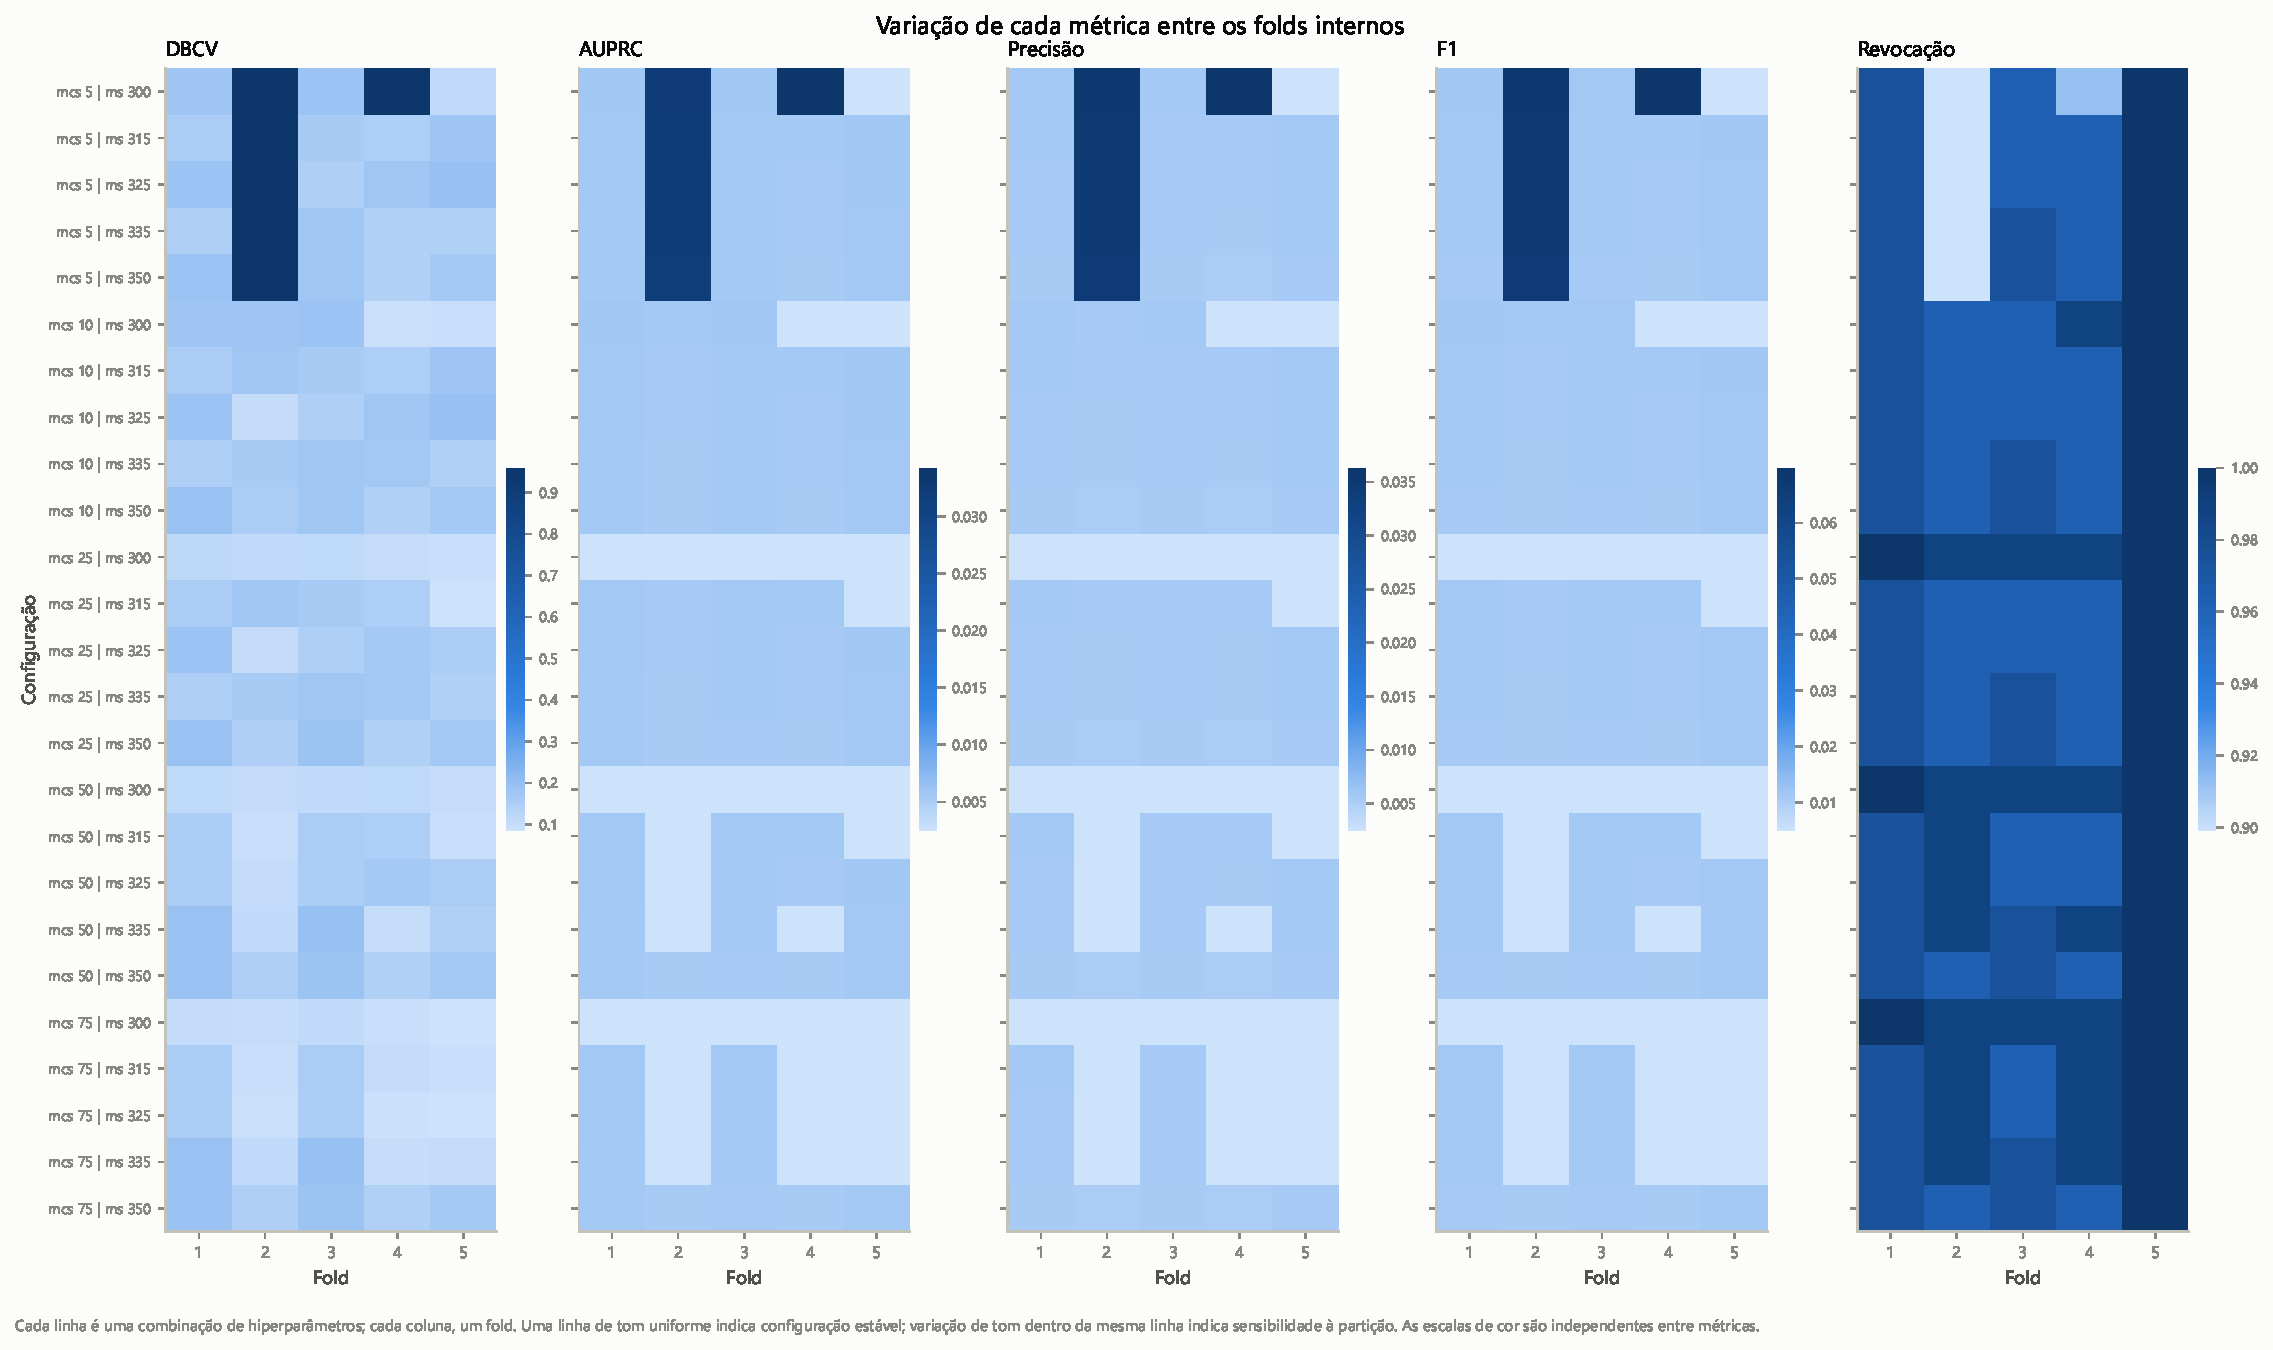
\includegraphics[width=\textwidth]{01-metric-stability.pdf}
    \caption{Valor de cada métrica para cada combinação de hiperparâmetros, em
    cada fold interno. Escalas de cor independentes entre métricas.}
\end{figure}

\textbf{Como ler.} Cada linha é uma combinação de hiperparâmetros; cada coluna,
um fold. Uma linha de tom uniforme indica configuração estável; variação de tom
dentro da mesma linha indica sensibilidade à partição.

\textbf{O que mostra.} A maior parte do painel é uniforme. A exceção está
concentrada nas linhas de \texttt{min\_cluster\_size}${}=5$, onde a coloração
muda bruscamente entre colunas.

\textbf{O que significa.} A substituição da figura anterior, que mostrava apenas
AUC ROC e tinha títulos sobrepostos, permite ver o que estava oculto: a
instabilidade não afeta o método como um todo, mas uma região específica do
espaço de parâmetros.

\section{Amplitude do DBCV por configuração}

\begin{figure}[H]
    \centering
    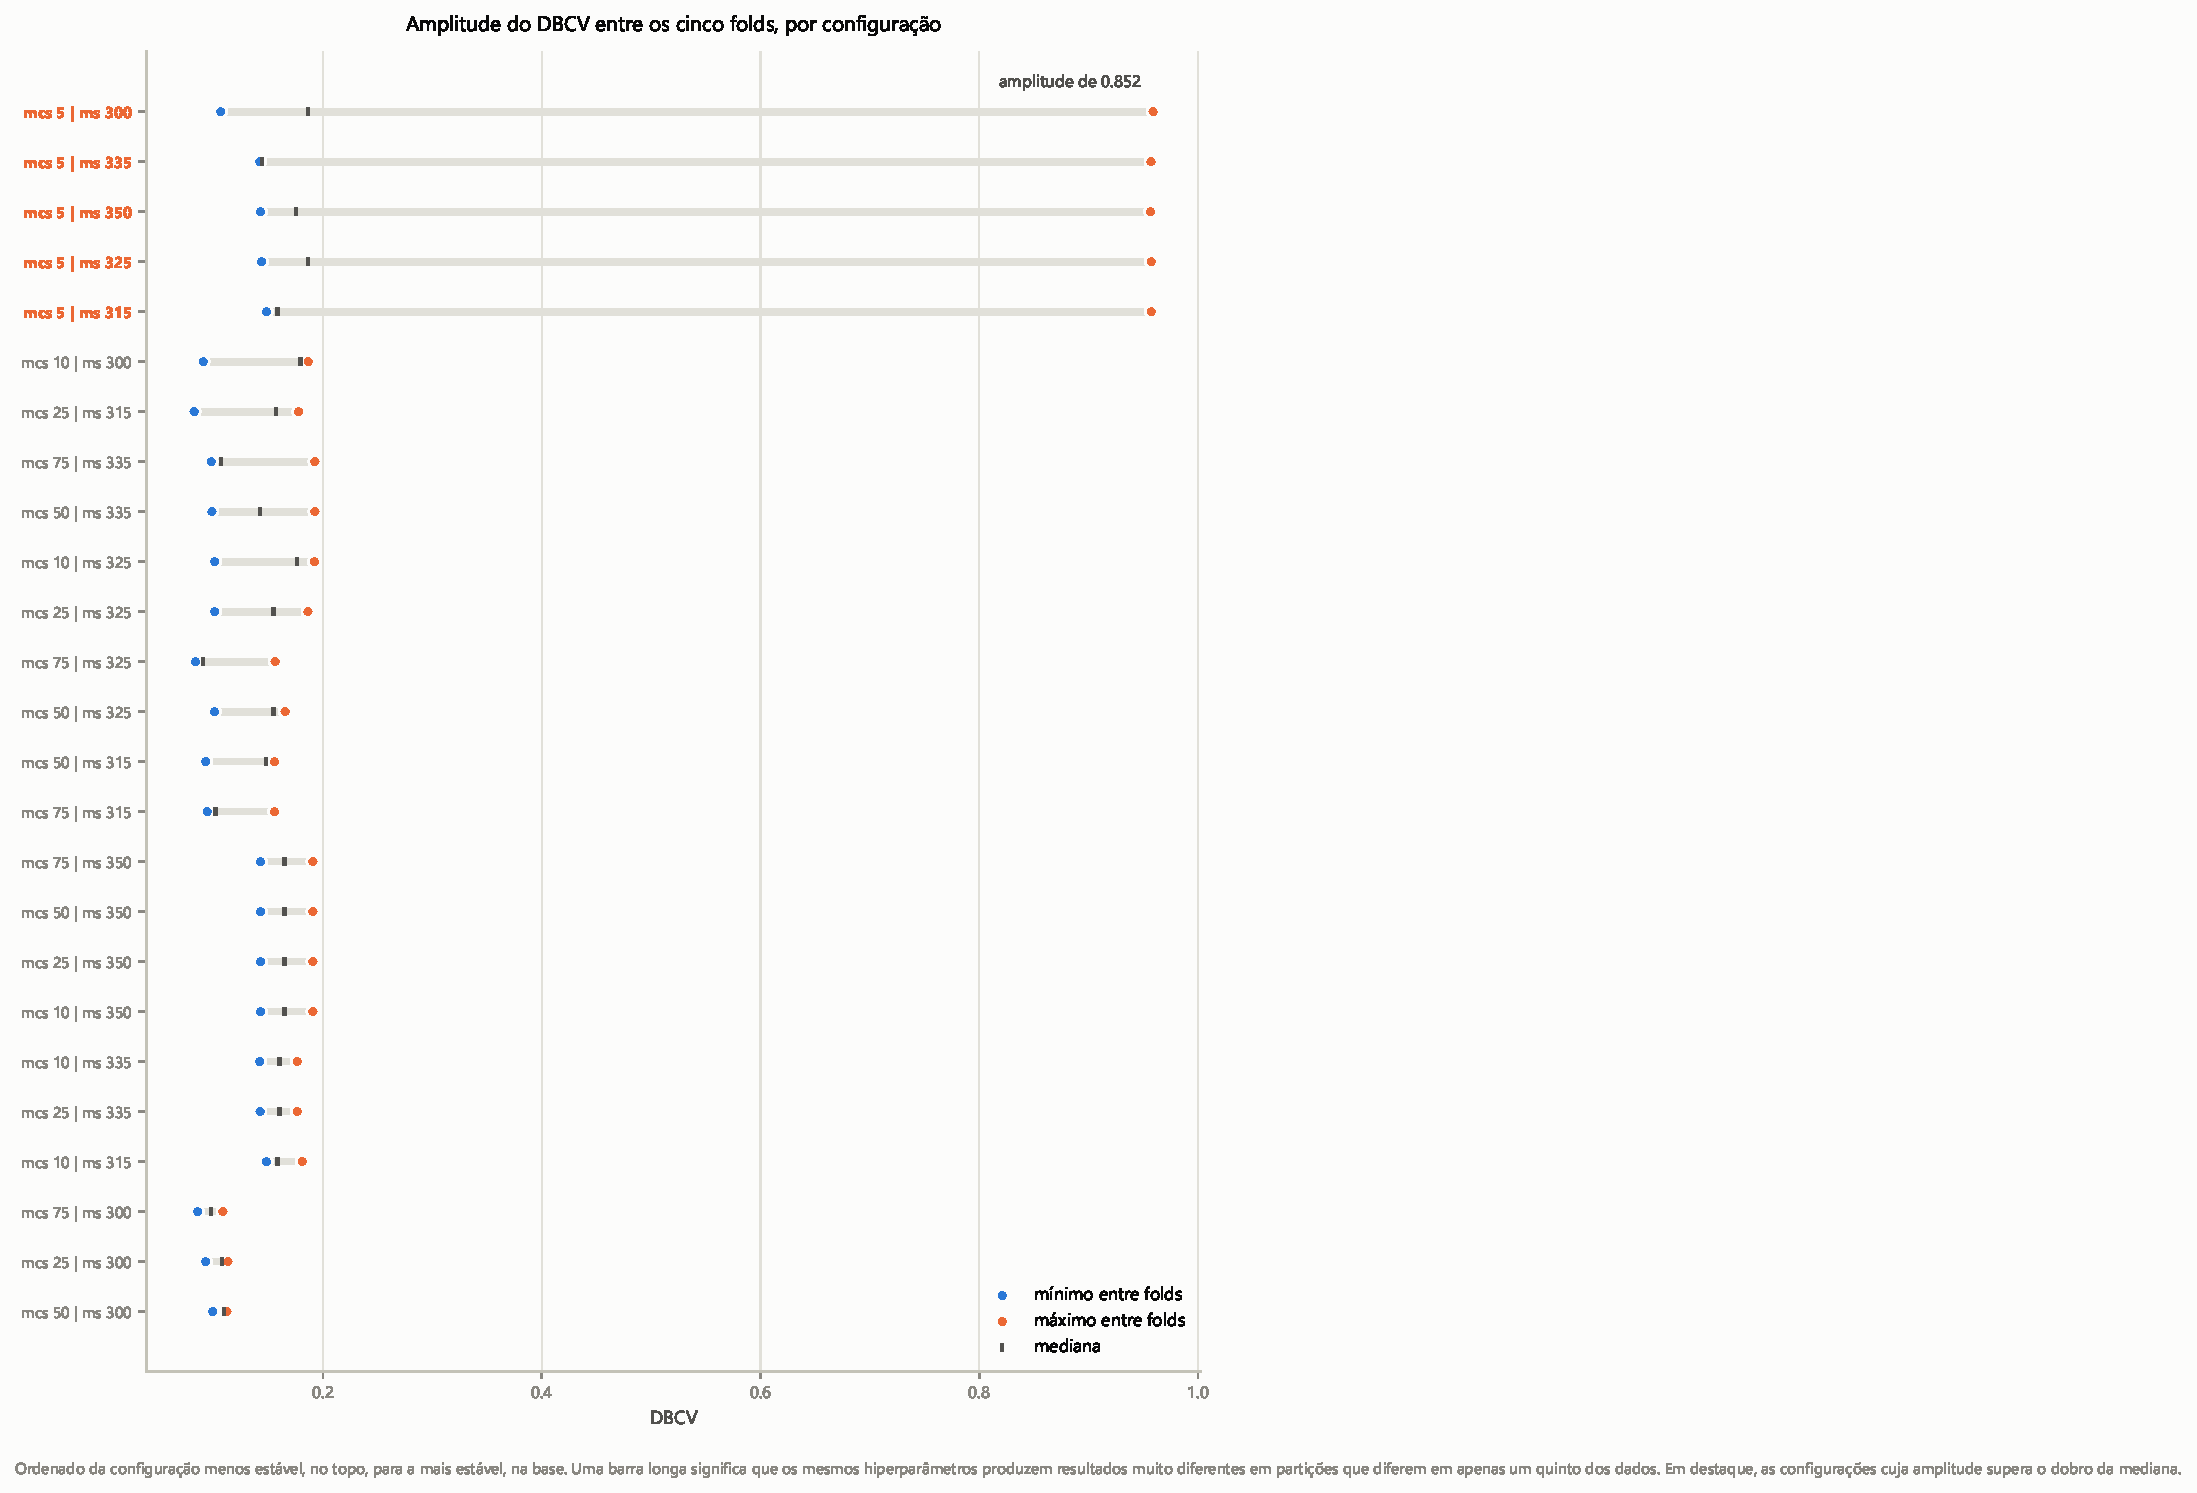
\includegraphics[width=0.92\textwidth]{02-dbcv-spread-by-config.pdf}
    \caption{Intervalo entre o menor e o maior DBCV obtido pela mesma
    configuração ao longo dos cinco folds, ordenado da menos estável para a mais
    estável.}
\end{figure}

\textbf{Como ler.} Cada barra horizontal vai do mínimo ao máximo observado.
Barra longa significa que os mesmos hiperparâmetros produziram resultados muito
diferentes. Os rótulos em destaque marcam as configurações cuja amplitude supera
o dobro da mediana.

\textbf{O que mostra.} A amplitude mediana é de apenas $0{,}065$. Mas as
\textbf{cinco configurações com \texttt{min\_cluster\_size}${}=5$} chegam a
$0{,}852$ --- o DBCV varia de $0{,}107$ a $0{,}959$ com os mesmos parâmetros. As
outras vinte configurações são estáveis.

\textbf{O que significa.} Combinando com a Parte II, o argumento fecha. As
partições são estruturalmente idênticas (razão de densidade entre $2{,}93\times$
e $3{,}03\times$), e ainda assim o DBCV oscila de $0{,}107$ a $0{,}959$ sobre
elas. A instabilidade, portanto, \textbf{é do algoritmo, não dos dados}.

O problema prático é que essa região instável é justamente a que vence a seleção
por DBCV.

\section{O DBCV prediz o desempenho?}

\begin{figure}[H]
    \centering
    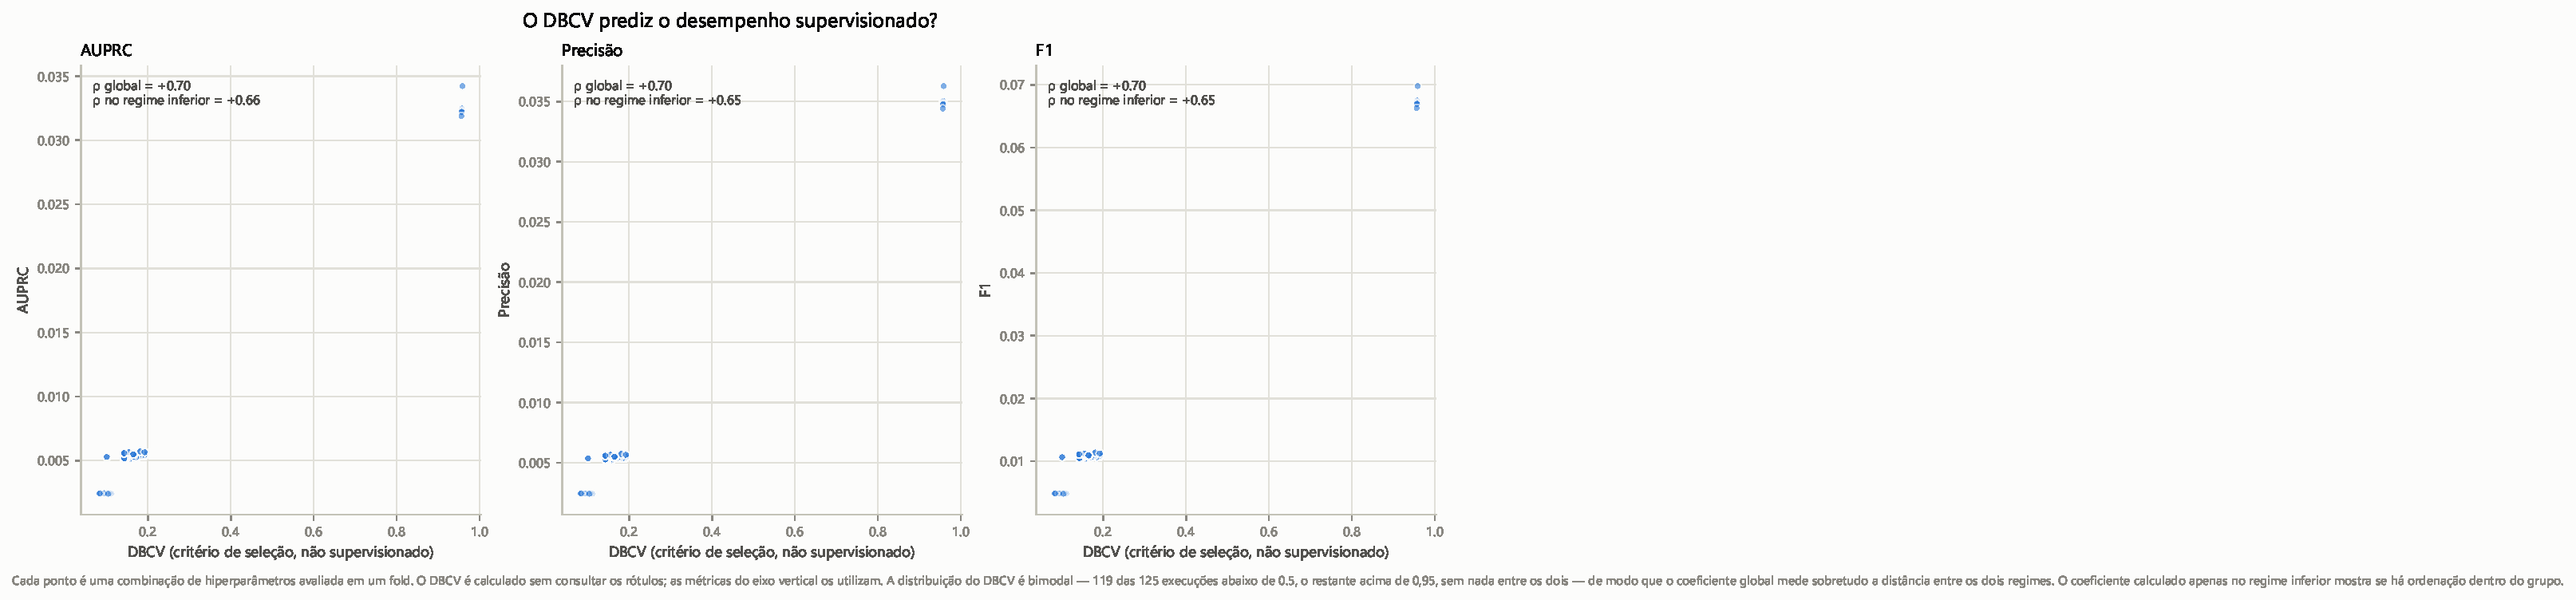
\includegraphics[width=\textwidth]{03-dbcv-vs-performance.pdf}
    \caption{DBCV --- calculado sem consultar os rótulos --- contra métricas
    supervisionadas. Cada ponto é uma combinação avaliada em um fold.}
\end{figure}

\textbf{Como ler.} O eixo horizontal traz o critério de seleção, que não usa
rótulos; o vertical, métricas que os utilizam. Correlação positiva indica que o
critério aponta na mesma direção do desempenho real.

\textbf{O que mostra.} O $\rho$ de Spearman global é de $+0{,}70$ com AUPRC, com
$p$ da ordem de $10^{-20}$.

\textbf{Uma ressalva que a figura torna visível.} A distribuição do DBCV é
\textbf{bimodal}: um grupo denso abaixo de $0{,}2$ e um grupo destacado acima de
$0{,}95$, sem nenhuma observação entre os dois. Um coeficiente único calculado
sobre os dois grupos mede sobretudo a distância entre eles, e não uma ordenação
gradual.

Por isso cada painel reporta também o coeficiente calculado \emph{apenas dentro
do regime inferior}: $\rho = +0{,}66$ com AUPRC, $p \approx 10^{-16}$.

\textbf{O que significa.} A relação se sustenta nas duas leituras. O DBCV
distingue corretamente os dois regimes \emph{e} ordena configurações dentro do
regime dominante. Isso justifica seu uso como critério de seleção sem vazamento
de rótulos --- e a ressalva sobre a bimodalidade precisa acompanhar o número
sempre que ele for reportado.

\clearpage
\section*{Síntese}

\begin{table}[H]
    \centering
    \small
    \begin{tabular}{p{5.4cm} p{10.2cm}}
        \toprule
        \textbf{Pergunta} & \textbf{Resposta} \\
        \midrule
        As componentes do PCA exigem tratamento de multicolinearidade? &
        Não. Correlação absoluta máxima de $2{,}32 \times 10^{-14}$ entre elas. \\
        \addlinespace
        A variável \texttt{Time} é relevante? &
        Como ordenador, não: lift de $1{,}43\times$, 27ª de 30. Como fator de
        risco a priori, sim: $5{,}6\times$ mais fraude entre 03h e 06h. \\
        \addlinespace
        Fraudes ocupam regiões de baixa densidade? &
        Sim. Distância mediana ao 20º vizinho $3{,}06\times$ maior
        ($D = 0{,}793$). \\
        \addlinespace
        A estratificação se manteve? &
        Sim. Proporção de fraude entre $0{,}1720\%$ e $0{,}1738\%$. \\
        \addlinespace
        Cada transação é testada uma única vez? &
        Sim. 284.807 transações, sobreposição nula entre conjuntos de teste. \\
        \addlinespace
        O HDBSCAN é instável? &
        Apenas em \texttt{min\_cluster\_size}${}=5$. Amplitude mediana de
        $0{,}065$; nessa região, $0{,}852$. \\
        \addlinespace
        A instabilidade vem dos dados ou do algoritmo? &
        Do algoritmo. A razão de densidade das partições varia só de
        $2{,}93\times$ a $3{,}03\times$. \\
        \addlinespace
        O DBCV é um critério de seleção defensável? &
        Sim, com ressalva. $\rho = +0{,}70$ global e $+0{,}66$ dentro do regime
        inferior, mas a distribuição é bimodal. \\
        \bottomrule
    \end{tabular}
\end{table}

\end{document}
